\documentclass[10pt,svgnames]{beamer}
\graphicspath{{images/}}
\usepackage[utf8]{inputenc}
\usepackage[english,russian]{babel}
\usepackage{booktabs}
\usepackage{biblatex}


\mode<presentation>
{
  \usetheme[titleformat=smallcaps,numbering=fraction,progressbar=frametitle]{metropolis}
  \usecolortheme[light,accent=orange]{solarized}
  %\usecolortheme[named=Goldenrod]{structure}
  % or ...

  \setbeamercovered{transparent}
  % or whatever (possibly just delete it)
}


\newcommand{\dir}{\text{Dirichlet}}
\newcommand{\mult}{\text{Multinomial}}
\usetikzlibrary{arrows,decorations.pathmorphing,fit,positioning}
\addbibresource{local.bib}



\title[QTA 08] % (optional, use only with long paper }
{Тематическое моделирование}

\subtitle
{Квантитативный анализ текста} % (optional)

\author%[Author, Another] % (optional, use only with lots of authors)
{Кирилл Александрович Маслинский}
% - Use the \inst{?} command only if the authors have different
%   affiliation.

\institute%[Universities of Somewhere and Elsewhere] % (optional, but mostly needed)
{ЕУСПб}
% - Use the \inst command only if there are several affiliations.
% - Keep it simple, no one is interested in your street address.

\date%[Short Occasion] % (optional)
{25.04.2022 / 08}

\subject{natural language processing, text mining}
% This is only inserted into the PDF information catalog. Can be left
% out. 



% If you have a file called "university-logo-filename.xxx", where xxx
% is a graphic format that can be processed by latex or pdflatex,
% resp., then you can add a logo as follows:

% \pgfdeclareimage[height=0.5cm]{university-logo}{university-logo-filename}
% \logo{\pgfuseimage{university-logo}}

% Delete this, if you do not want the table of contents to pop up at
% the beginning of each subsection:

\newcommand{\plate}[1]{\begingroup\setbeamercolor{background canvas}{bg=Beige}
  % \begin{frame}<beamer>{Outline}
  %   \tableofcontents[sectionstyle=show/hide,subsectionstyle=show/shaded/hide]
  % \end{frame}
  \begin{frame}[plain]
  \vfill
  \centering
  \begin{beamercolorbox}[sep=8pt,center,shadow=true,rounded=true]{title}
    \usebeamerfont{title}#1\par%
  \end{beamercolorbox}
  \vfill
  \end{frame}
  \endgroup
}

% \AtBeginSection[]
% {
%   \begin{frame}<beamer>[plain]{План}
%     \tableofcontents[sectionstyle=shaded,subsectionstyle=hide]
%   \end{frame}
% }

% \AtBeginSubsection[]
% {
%   \begin{frame}<beamer>[plain]{План}
%     \tableofcontents[sectionstyle=shaded,subsectionstyle=show]
%   \end{frame}
% }

\newcommand{\tb}[1]{\colorbox{yellow}{#1}\space}
\newcommand{\Sp}[1]{\colorbox{green}{#1}\space}
\newcommand{\Sn}[1]{\colorbox{red}{#1}\space}


\begin{document}

\begin{frame}
  \titlepage
\end{frame}

\section{От слов к темам}

\subsection{Multinomial distribution}

\begin{frame}
  \frametitle{Multinomial distribution over words}

  \begin{block}{Исходный текст}
    Карл у Клары украл кораллы, Клара у Карла украла кларнет.
  \end{block}
  
  \begin{block}{Словарь (распределение)}
    \begin{tabular}[c]{cccccc} 
      Карл&у&Клара&украсть&коралл&кларнет\\
      Карл&у&Клара&украсть&      &       \\ 
      2 & 2& 2 & 2& 1& 1\\
      0.2 & 0.2 & 0.2 & 0.2 & 0.1 & 0.1 \\
    \end{tabular}
  \end{block}
\end{frame}

\begin{frame}
  \frametitle{Корпус как смесь тем (распределений)}
  \footnotesize
  \begin{block}{Темы — события}
    \begin{tabular}[c]{lccccccr}
      Тема &&&&&&& всего \\
      \hline
      & Карл&у&Клара&украсть&коралл&кларнет&\\
     \textit{Карл}& 0,1 & 0,1 & 0,1 & 0,1 & 0,1 & \alert{0} & \textbf{0,5} \\
      \textit{Клара} & 0,1 & 0,1 & 0,1 & 0,1 & \alert{0} & 0,1 & \textbf{0,5}\\
    \end{tabular}
  \end{block}

  \begin{block}{Темы — общее и различное}
    \begin{tabular}[c]{lccccccr}
      Тема &&&&&&& всего \\
      \hline
      & Карл&у&Клара&украсть&коралл&кларнет&\\
     \textit{Общее} & 0,2 & 0,2 & 0,2 & 0,2 & 0 & 0 & \textbf{0,8}\\
      \textit{Разное} & 0 & 0 & 0 & 0 & 0,1 & 0,1 & \textbf{0,2}\\ 
    \end{tabular}
  \end{block}
\end{frame}

\subsection{Переходная форма: Вероятностный LSA}

\begin{frame}
  \frametitle{Probabilistic Latent semnatic analysis (pLSA)}
  Hoffman 1999

  Тема:
  \begin{itemize}
  \item \alert{латентная} переменная (объясняет распределение слов в корпусе)
  \item представляет собой мультиномиальное распределение
  \end{itemize}
\end{frame}

\begin{frame}
  \frametitle{Порождающие вероятностные модели}
  \framesubtitle{Generative probabilistic model}
  \begin{enumerate}
  \item Предположим, что тексты сгенерированы с помощью случайного
    процесса, у которого есть \alert{параметры}.
  \item \alert{Подберем} значения параметров, которые наилучшим
    образом объясняют наши данные (предсказывают, что будут
    сгенерированы именно такие тексты).
  \item Используем модель, чтобы \alert{предсказывать} новые данные,
    основываясь на уже виденных.
  \end{enumerate}
\end{frame}

\begin{frame}
  \frametitle{Генеративная модель pLSA}
    Для каждого \structure{слова} в каждом документе:
  \begin{enumerate}
  \item Выбрать <случайным образом> тему $z$ на основании
    распределения вероятностей тем в коллекции.
  \item Выбрать <случайным образом> слово на основании распределения
    вероятностей слов в теме $z$.
  \end{enumerate}
  Свойства:
  \begin{itemize}
  \item у каждого слова — одна тема;
  \item в документе может быть несколько тем;
  \item в коллекции — одно общее распределение вероятностей тем.
  \end{itemize}
\end{frame}

\begin{frame}
  \frametitle{Графическая модель pLSA}
  \centering
  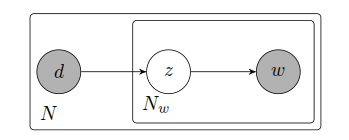
\includegraphics[width=\textwidth]{plsa-model}
\end{frame}

\subsection{Latent Dirichlet Allocation}

\begin{frame}
  \frametitle{LDA — Модель}
  Предположим:
  \begin{itemize}
  \item В коллекции представлено $K$ тем.
  \item Каждый документ представляет собой \structure{смесь тем}.
  \item «Тема» — мультиномиальное распределение слов. Каждое слово в
    словаре имеет определенный вес (вероятность) \structure{в каждой теме}.
  \end{itemize}

  Свойства:
  \begin{itemize}
  \item У документа может быть несколько тем.
  \item У каждого слова — одна тема.
  \item У каждого документа в коллекции — свое распределение тем (в
    одном документе представлены только \structure{некоторые} темы коллекции).
  \end{itemize}
\end{frame}

\begin{frame}
  \frametitle{Порождающий процесс для LDA}
  \begin{itemize}
  \item[для] каждого документа $d_d$ в корпусе $D$
  \item[Шаг:] Выбрать $\theta_d \sim \dir(\alpha) $
  \item[для] каждой позиции $w$ в документе $d_d$
    \begin{itemize}
    \item[Шаг:] Выбрать тему $z_w \sim \mult(\theta_d)$
    \item[Шаг:] Выбрать слово $w_w$ из $p(w_w | z_w,\beta)$,
    \end{itemize}
    мультиномиального распределения над словами, зависящего от темы и $\beta$.
  % \ENDFOR
  % \ENDFOR
\end{itemize}
\end{frame}


\begin{frame}
  \frametitle{Графическая модель LDA}
  \centering
  \begin{tikzpicture}
    [
      observed/.style={minimum size=15pt,circle,draw=blue!50,fill=blue!20},
      unobserved/.style={minimum size=15pt,circle,draw},
      hyper/.style={minimum size=1pt,circle,fill=black},
      post/.style={->,>=stealth',semithick},
    ]

    \node (w-j) [observed] at (0,0) {$w_w$};
    \node (z-j) [unobserved] at (-1.5,0) {$z_w$};
    \node (z-prior) [unobserved] at (-3,0) {$\theta_d$};
    \node (z-hyper) [label=above:$\alpha$] at (-4.5,0) {};
    \filldraw [black] (-4.5,0) circle (3pt);
    \node (w-hyper) [label=above:$\beta$] at (-1.5,1.5) {};
    \filldraw [black] (-1.5,1.5) circle (3pt);
    
    \path
    (z-j) edge [post] (w-j)
    
    (z-hyper) edge [post] (z-prior)
    (z-prior) edge [post] (z-j)

    (w-hyper) edge [post] (w-j)
    ;

    \node [draw,fit=(w-j) (z-prior), inner sep=14pt] (plate-context) {};
    \node [above right] at (plate-context.south west) {$D$};
    \node [draw,fit=(w-j) (z-j), inner sep=10pt] (plate-token) {};
    \node [above right] at (plate-token.south west) {$N$};
  \end{tikzpicture}
  \label{fig:graphical-model}
\end{frame}

\begin{frame}[plain]
  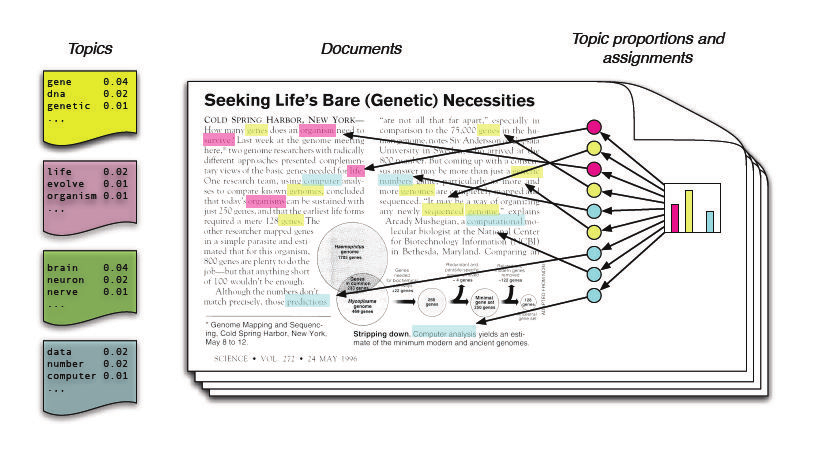
\includegraphics[width=\textwidth]{blei-slide}

  \footnotesize 

  Slide by David Blei
\end{frame}


\section{Тематическое моделирование: процедура}

\subsection{Препроцессинг}

\begin{frame}
  \frametitle{Стоп-слова}
  \begin{itemize}
  \item Статический список:
без
более
бы
был
была
были
было
быть
в
вам
вас
весь
во
вот
все
всего
всех
вы
где
да
даже
для ...

  \item Динамический список:

    \begin{itemize}
    \item Слишком частотные (N самых частотных)
    \item Слишком редкие (порог: не менее чем в F документов)
    \item Слишком короткие (меньше M букв)
    \item Не существительные
    \item Имена собственные
    \end{itemize}
  \end{itemize}
\end{frame}

\subsection{Сегментация}

\begin{frame}
  \frametitle{Размер документа имеет значение}
  \begin{itemize}
  \item Разбиение длинных текстов — романы
  \item Объединение коротких текстов — сообщения в чате
  \item Оптимальный(?) масштаб — 100—1000 слов (от абстракта до статьи)
  \end{itemize}
  \centering
  \alert{Главный принцип — единство контекста.}
\end{frame}

\subsection{Расчет модели}

\begin{frame}
  \frametitle{Черная магия с разоблачением}
  \begin{itemize}
  \item Мы не можем наблюдать «темы».
  \item Мы наблюдаем только документы.
  \item LDA должен «восстановить» \structure{дискурсы}, которые
    породили документы.
  \item Невозможно точно восстановить темы: слишком много неизвестных.
  \end{itemize}
\end{frame}

\begin{frame}
  \frametitle{Gibbs sampling}
  \begin{block}{Представим, что мы почти решили проблему:}
    Мы знаем, к какой теме принадлежит каждое слово коллекции,
    \structure{кроме одного слова}. 
  \end{block}
  
  Как решить, к какой теме принадлежит это слово?
\end{frame}

\begin{frame}
  \frametitle{Gibbs sampling}
  Рассмотрим два вопроса (для каждой темы Z):
  \begin{enumerate}
  \item \structure{Как часто слово принадлежит к теме Z?}

    Если данное слово часто возникает при обсуждении Z, то и
    рассматриваемое словоупотребление может относиться к Z.
  \item \structure{Насколько часто тема Z встречается в этом документе?} 

    Cколько слов документа отнесено к теме Z. Если Z уже обсуждается в
    данном документе, вероятно, что и данное слово к ней относится.
  \end{enumerate}
\end{frame}

\begin{frame}
  \frametitle{[Collapsed] Gibbs sampling}
  $$
  P(Z|W,D) = \frac{\text{частотность W в Z} + \beta_w}{\text{всего
      словоупотреблений в Z} + \beta} \cdot (\text{слов из Z в D} + \alpha)
  $$

  \begin{itemize}
  \item[Z] — тема;
  \item[W] — слово;
  \item[D] — документ;
  \item[$\alpha,\beta$] — гиперпараметры. Позволяют учесть вероятность,
  что W может относиться к Z, даже если оно там раньше не встречалось.
  \end{itemize}
\end{frame}


\begin{frame}
  \frametitle{Collapsed Gibbs sampling}
  \begin{enumerate}
  \item Назначаем всем словам в коллекции произвольные темы.
  \item Поочередно для каждого слова заново <случайным образом>
    выбираем тему в соответствии с вероятностями тем для этого слова,
    вычисленными по приведенной выше формуле.
  \end{enumerate}
  Модель будет постепенно улучшаться, так что:
  \begin{itemize}
  \item Слова будут все чаще относиться к темам, где они уже
    распространены.
  \item Темы, которые распространены в документе, будут
    распространяться в нем еще.
  \end{itemize}
  \structure{Принцип: Rich get richer}
\end{frame}

\subsection{Интерпретация}

\begin{frame}
  \footnotesize
  \begin{block}{Фрида Вигдорова, Это мой дом (1961)}
Меня вызвали в <>. Я шел по длинному \textcolor{orange}{полутемному коридору}, и вдруг
откуда-то \textcolor{orange}{выскочила} девчонка лет одиннадцати.

<...>

Вызвала меня <>. Когда я \textcolor{orange}{вошел}, она бегло
посмотрела в мою сторону, уронила: <...> – Привычку командовать надо
оставить, то-ва-рищ <>! Я вижу, что слухи о вашем самомнении не
преувеличены. Я вызвала вас для того, чтобы сказать: неприлично
\textcolor{cyan}{директору} детдома заниматься саморекламой!

И вот тут я делаю непозволительную глупость. При этом имени я встаю и,
не прощаясь, покидаю кабинет <>. <...>
Иду по \textcolor{orange}{коридору}, стиснув зубы, и злюсь на себя.

Оборачиваюсь. Девчонка со всех ног \textcolor{orange}{удирает} от меня и, еще два раза
выкрикнув ехидным голосом: «Цыган! Цыган!» – \textcolor{orange}{скрывается за дверью} в
конце \textcolor{orange}{коридора}.

– Ну нет! Не уйдешь!

Иду за ней, дергаю \textcolor{orange}{дверь} – она \textcolor{orange}{заперта} изнутри. Стою тихо, жду. \textcolor{orange}{Дверь
чуть приоткрывается}, \textcolor{orange}{в щелку} виден кончик вздернутого носа, и \textcolor{orange}{дверь
снова захлопывается}.
  \end{block}
\end{frame}

\begin{frame}
  \frametitle{Гадание на темах}
  \begin{columns}
    \column{0.3\textwidth}
    \includegraphics<1>[width=.95\textwidth]{tealeafreading}
    \includegraphics<2>[width=.95\textwidth]{trelawney}
    \column{0.7\textwidth}
    \fullcite{chang2009reading}
  \end{columns}
\end{frame}

\begin{frame}
  \only<2->{
    \begin{columns}
      \column{.25\textwidth}
      
\includegraphics[width=\textwidth]{snape}
      \column{.75\textwidth}
      {\centering\LARGE\alert{Интерпретация:\\ \only<3>{портретные описания}}\par}
    \end{columns}
}

\bigskip

  \textcolor<2>{orange}{глаз} \textcolor<3>{cyan}{лицо губа рука} \textcolor<2>{orange}{взгляд} \textcolor<3>{cyan}{бровь волос голос улыбка нос лоб}
  \textcolor<2>{orange}{взглядывать} \textcolor<3>{cyan}{щека} \textcolor<2>{orange}{подымать} темный \textcolor<3>{cyan}{плечо} \textcolor<2>{orange}{строгий} широкий \textcolor<3>{cyan}{рот}
  повертываться черный \textcolor<3>{cyan}{ухо палец} открытый словно \textcolor<2>{orange}{выражение} высокий
  бледный густой весить прямой \textcolor<3>{cyan}{подбородок} звать угол чувствовать
  круглый вспыхивать похожий покраснеть сводить слегка несколько
  спокойно дело \textcolor<3>{cyan}{ресница} левый живой поглядеть успевать  
\end{frame}

\section{Оценка качества и подбор параметров модели}

\subsection{Метрики качества тем}

\begin{frame}
  \frametitle{Разновидности неудачных тем}
  \footnotetext{\fullcite{mimno2011optimizing}}
  \begin{description}
  \item[Chained] every word is connected to every other word through
    some pairwise word chain, but not all word pairs make sense.

    \alert{fatty $\leftarrow$ acids $\rightarrow$ nucleic}
  \item[Intruded] either two or more unrelated sets of related words,
    joined arbitrarily, or an otherwise good topic with a few
    “intruder” words.
  \item[Random] no clear, sensical connections between more than a few
    pairs of words
  \item[Unbalanced] the top words are all logically connected to each
    other, but the topic combines very general and specific terms
  \end{description}
\end{frame}

\begin{frame}
  \frametitle{Topic size}
  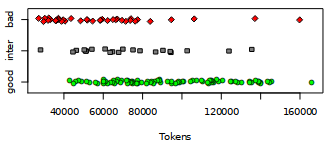
\includegraphics[width=\textwidth]{topicsize}
\end{frame}

\begin{frame}
  \frametitle{Topic coherence}
  $$
  C(t; V^{(t)}) =\sum_{m=2}^{M} \sum_{l=1}^{m-1} \log\frac{D(w_{m}^{(t)},w_{l}^{(t)})+1}{D(w_{l}^{(t)})}
  $$, где
  \begin{itemize}
  \item $D(w)$ — документная частота слова $w$
  \item $D(w,w')$ — совместная документная частота слов $w$ и $w'$
  \item $V^{(t)}=(v_1^{(t)},\dots, v_M^{(t)})$ — список M самых вероятных слов в теме t
  \end{itemize}
\end{frame}

\begin{frame}
  \frametitle{Topic coherence}
  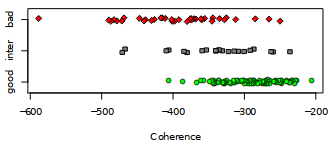
\includegraphics[width=\textwidth]{coherence}
\end{frame}

\subsection{Количество тем}

\begin{frame}
  \frametitle{Чему равно K (количество тем)?}
  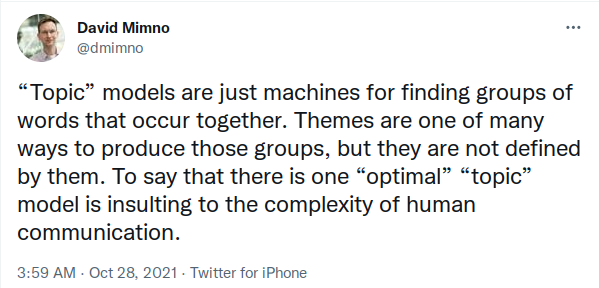
\includegraphics[width=\textwidth]{dmimno-on-tm}
\end{frame}


  \section{Summary}

  \begin{frame}
    \frametitle{LDA: Итоговый рецепт}
    \begin{columns}
      \column{.3\textwidth}
      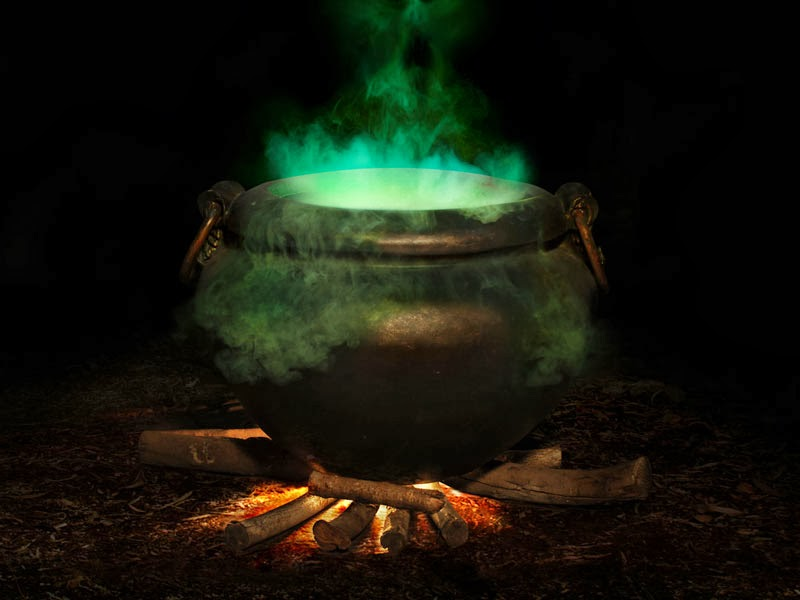
\includegraphics[width=\textwidth]{potion}
      \column{.7\textwidth}
      \begin{itemize}
      \item Дистрибутивная гипотеза
      \item Корпус текстов
      \item Границы документов
      \item Отбор и нормализация слов
      \item Матрица термов-документов
      \item Тема как мультиномиальное распределение над словами
      \item Модель распределения тем в документах по Дирихле
      \item Collapsed Gibbs Sampling
      \item Интерпретация
      \end{itemize}
    \end{columns}
  \end{frame}

\end{document}
